\section{Tree comparison}
\subsection{Necessary knowledge - Splitting}
Where can we split this tree? 
\begin{figure}[H]
    \centering
    \begin{tikzpicture}
\path node (A) at (1.4,3.4) {A}
node (DAF) at (0,0) {}
node (DA) at (0,2) {}
node (D) at (-0.7,2.7) {D}
node (F) at (-1,0) {F}
node (EG) at (2.1,-2.1) {}
node (G) at (3.5,-3.5) {G}
node (E) at (1.4,-2.8) {E}
node (BC) at (4,0) {}
node (C) at (5.5, 0) {C}
node (B) at (4,2) {B}
;
\draw   (DAF) -- (F);
\draw   (DA) -- (DAF);
\draw   (A) -- (DA);
\draw   (D) -- (DA);
\draw   (EG) -- (DAF);
\draw   (EG) -- (G);
\draw   (EG) -- (E);
\draw   (EG) -- (BC);
\draw   (B) -- (BC);
\draw   (C) -- (BC);
\end{tikzpicture}
    \caption{Example tree.}
    \label{fig:my_label}
\end{figure}
We cannot split edges that connect directly to a tree. (Or rather we can, but they are trivial splits and unnecessary.) 
\begin{figure}[H]
    \centering
    \begin{tikzpicture}
\path node (A) at (1.4,3.4) {A}
node (DAF) at (0,0) {}
node (DA) at (0,2) {}
node (D) at (-0.7,2.7) {D}
node (F) at (-1,0) {F}
node (EG) at (2.1,-2.1) {}
node (G) at (3.5,-3.5) {G}
node (E) at (1.4,-2.8) {E}
node (BC) at (4,0) {}
node (C) at (5.5, 0) {C}
node (B) at (4,2) {B}
;
\draw[red]   (DAF) -- (F);
\draw   (DA) -- (DAF);
\draw[red]   (A) -- (DA);
\draw[red]   (D) -- (DA);
\draw   (EG) -- (DAF);
\draw[red]   (EG) -- (G);
\draw[red]   (EG) -- (E);
\draw   (EG) -- (BC);
\draw[red]   (B) -- (BC);
\draw[red]   (C) -- (BC);
\end{tikzpicture}
    \caption{Visualisation which edges cannot be used to split the example tree.}
    \label{fig:my_label}
\end{figure}


This leaves three possible splits
\begin{figure}[H]
    \centering 
\begin{subfigure}[t]{0.3\textwidth}
      \resizebox{4cm}{!}{
    \begin{tikzpicture}
\path node (A) at (1.4,3.4) {A}
node (DAF) at (0,0) {}
node (DA) at (0,2) {}
node (D) at (-0.7,2.7) {D}
node (F) at (-1,0) {F}
node (EG) at (2.1,-2.1) {}
node (G) at (3.5,-3.5) {G}
node (E) at (1.4,-2.8) {E}
node (BC) at (4,0) {}
node (C) at (5.5, 0) {C}
node (B) at (4,2) {B}
;
\draw   (DAF) -- (F);
\draw   (A) -- (DA);
\draw   (D) -- (DA);
\draw   (EG) -- (DAF);
\draw   (EG) -- (G);
\draw   (EG) -- (E);
\draw   (EG) -- (BC);
\draw   (B) -- (BC);
\draw   (C) -- (BC);
\end{tikzpicture}
      }
    \end{subfigure}
    \hfill
    \begin{subfigure}[t]{0.3\textwidth}
      \resizebox{4cm}{!}{
    \begin{tikzpicture}
\path node (A) at (1.4,3.4) {A}
node (DAF) at (0,0) {}
node (DA) at (0,2) {}
node (D) at (-0.7,2.7) {D}
node (F) at (-1,0) {F}
node (EG) at (2.1,-2.1) {}
node (G) at (3.5,-3.5) {G}
node (E) at (1.4,-2.8) {E}
node (BC) at (4,0) {}
node (C) at (5.5, 0) {C}
node (B) at (4,2) {B}
;
\draw   (DAF) -- (F);
\draw   (DA) -- (DAF);
\draw   (A) -- (DA);
\draw   (D) -- (DA);
\draw   (EG) -- (G);
\draw   (EG) -- (E);
\draw   (EG) -- (BC);
\draw   (B) -- (BC);
\draw   (C) -- (BC);
\end{tikzpicture}
      }
    \end{subfigure}
    \hfill
    \begin{subfigure}[t]{0.3\textwidth}
      \resizebox{4cm}{!}{
    \begin{tikzpicture}
\path node (A) at (1.4,3.4) {A}
node (DAF) at (0,0) {}
node (DA) at (0,2) {}
node (D) at (-0.7,2.7) {D}
node (F) at (-1,0) {F}
node (EG) at (2.1,-2.1) {}
node (G) at (3.5,-3.5) {G}
node (E) at (1.4,-2.8) {E}
node (BC) at (4,0) {}
node (C) at (5.5, 0) {C}
node (B) at (4,2) {B}
;
\draw   (DAF) -- (F);
\draw   (DA) -- (DAF);
\draw   (A) -- (DA);
\draw   (D) -- (DA);
\draw   (EG) -- (DAF);
\draw   (EG) -- (G);
\draw   (EG) -- (E);
\draw   (B) -- (BC);
\draw   (C) -- (BC);
\end{tikzpicture}
      }
    \end{subfigure}
    
    \caption{Possible splits for the example tree.}
    \label{fig:my_label}
\end{figure}






\begin{figure}[H]
   \begin{subfigure}[t]{0.3\textwidth}
    \centering
      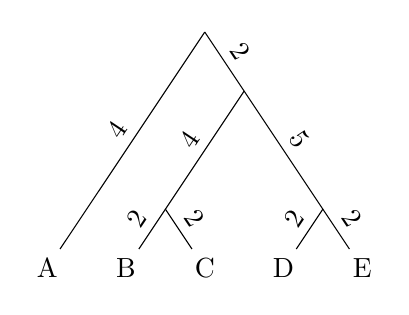
\begin{tikzpicture}
\pgftransformscale{.25}
   \node at (8,-12)  (E) {E};
   \node at (4,-12)  (D) {D};
   \node at (0,-12)  (C) {C};
    \node at (-4,-12)  (B) {B};
    \node at (-8,-12)  (A) {A};

    
    \draw (0,0)   -- (A) node[midway,sloped,above] {4};
  
    \draw (0,0)   -- (2,-3) node[midway,sloped,above] {2};
     \draw (2,-3)   -- (6,-9) node[midway,sloped,above] {5};
     \draw (6,-9)   -- (E) node[midway,sloped,above] {2};
   \draw (6,-9)   -- (D) node[midway,sloped,above] {2};
   \draw (2,-3)   -- (-2,-9) node[midway,sloped,above] {4};
   \draw (-2,-9)   -- (C) node[midway,sloped,above] {2};
   \draw (-2,-9)   -- (B) node[midway,sloped,above] {2};

    \end{tikzpicture}
    \subcaption{$T$}
   \end{subfigure}
    \hfill
   \begin{subfigure}[t]{0.3\textwidth}
    \centering
       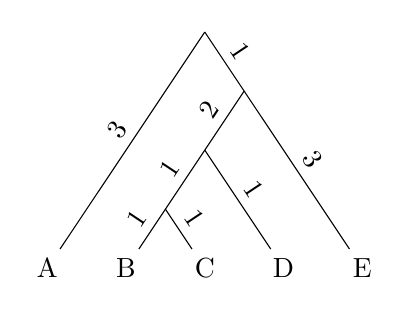
\begin{tikzpicture}
\pgftransformscale{.25}
   \node at (8,-12)  (E) {E};
   \node at (4,-12)  (D) {D};
   \node at (0,-12)  (C) {C};
    \node at (-4,-12)  (B) {B};
    \node at (-8,-12)  (A) {A};

    
    \draw (0,0)   -- (A) node[midway,sloped,above] {3};
  
    \draw (0,0)   -- (2,-3) node[midway,sloped,above] {1};
     \draw (2,-3)   -- (E) node[midway,sloped,above] {3};
     
     \draw (2,-3)   -- (0,-6) node[midway,sloped,above] {2};
     
     \draw (0,-6)   -- (-2,-9) node[midway,sloped,above] {1};
     
   \draw (0,-6)   -- (D) node[midway,sloped,above] {1};
   
   \draw (-2,-9)   -- (C) node[midway,sloped,above] {1};
   \draw (-2,-9)   -- (B) node[midway,sloped,above] {1};

    \end{tikzpicture}
    \subcaption{$T_1$}
   \end{subfigure}
 \hfill
   \begin{subfigure}[t]{0.3\textwidth}
   \centering
        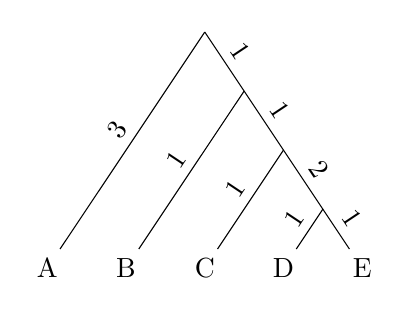
\begin{tikzpicture}
    
\pgftransformscale{.25}
   \node at (8,-12)  (E) {E};
   \node at (4,-12)  (D) {D};
   \node at (0,-12)  (C) {C};
    \node at (-4,-12)  (B) {B};
    \node at (-8,-12)  (A) {A};

    
    \draw (0,0)   -- (A) node[midway,sloped,above] {3};
  
    \draw (0,0)   -- (2,-3) node[midway,sloped,above] {1};
     \draw (2,-3)   -- (4,-6) node[midway,sloped,above] {1};
     \draw (4,-6)   -- (6,-9) node[midway,sloped,above] {2};
     \draw (6,-9)   -- (E) node[midway,sloped,above] {1};
 
     
   \draw (6,-9)   -- (D) node[midway,sloped,above] {1};
   
   \draw (4,-6)   -- (C) node[midway,sloped,above] {1};
   \draw (2,-3)   -- (B) node[midway,sloped,above] {1};

    \end{tikzpicture}
    \subcaption{$T_2$}
   \end{subfigure}

    \caption{Example trees to visualise distances.}
    \label{fig:splitexample}
\end{figure}


\subsection{Symmetric distance}
\begin{figure}[H]
   \begin{subfigure}[t]{0.45\textwidth}
    \centering
      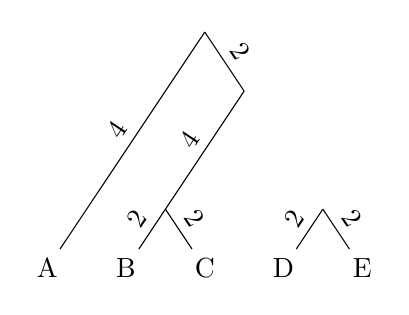
\begin{tikzpicture}
\pgftransformscale{.25}
   \node at (8,-12)  (E) {E};
   \node at (4,-12)  (D) {D};
   \node at (0,-12)  (C) {C};
    \node at (-4,-12)  (B) {B};
    \node at (-8,-12)  (A) {A};

    
    \draw (0,0)   -- (A) node[midway,sloped,above] {4};
  
    \draw (0,0)   -- (2,-3) node[midway,sloped,above] {2};
     \draw (6,-9)   -- (E) node[midway,sloped,above] {2};
   \draw (6,-9)   -- (D) node[midway,sloped,above] {2};
   \draw (2,-3)   -- (-2,-9) node[midway,sloped,above] {4};
   \draw (-2,-9)   -- (C) node[midway,sloped,above] {2};
   \draw (-2,-9)   -- (B) node[midway,sloped,above] {2};

    \end{tikzpicture}
    \subcaption{$\{A,B,C \mid D,E\}$}
   \end{subfigure}
   \hfill
    \begin{subfigure}[t]{0.45\textwidth}
    \centering
      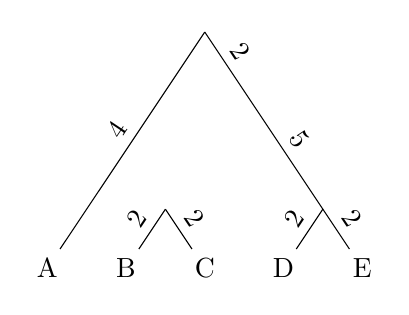
\begin{tikzpicture}
\pgftransformscale{.25}
   \node at (8,-12)  (E) {E};
   \node at (4,-12)  (D) {D};
   \node at (0,-12)  (C) {C};
    \node at (-4,-12)  (B) {B};
    \node at (-8,-12)  (A) {A};

    
    \draw (0,0)   -- (A) node[midway,sloped,above] {4};
  
    \draw (0,0)   -- (2,-3) node[midway,sloped,above] {2};
     \draw (2,-3)   -- (6,-9) node[midway,sloped,above] {5};
     \draw (6,-9)   -- (E) node[midway,sloped,above] {2};
   \draw (6,-9)   -- (D) node[midway,sloped,above] {2};
   \draw (-2,-9)   -- (C) node[midway,sloped,above] {2};
   \draw (-2,-9)   -- (B) node[midway,sloped,above] {2};

    \end{tikzpicture}
    \subcaption{$\{B,C \mid A,D,E\}$}
   \end{subfigure}
    \caption{Non-trivial splits of $T$.}
    \label{fig:splitst}
\end{figure}




\begin{figure}[H]
    \begin{subfigure}[t]{0.45\textwidth}
    \centering
       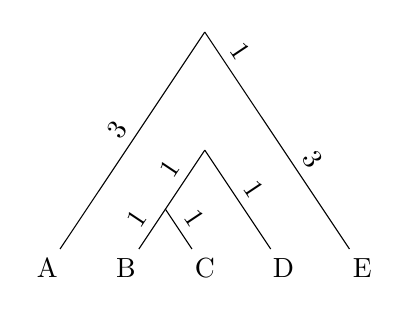
\begin{tikzpicture}
\pgftransformscale{.25}
   \node at (8,-12)  (E) {E};
   \node at (4,-12)  (D) {D};
   \node at (0,-12)  (C) {C};
    \node at (-4,-12)  (B) {B};
    \node at (-8,-12)  (A) {A};

    
    \draw (0,0)   -- (A) node[midway,sloped,above] {3};
  
    \draw (0,0)   -- (2,-3) node[midway,sloped,above] {1};
     \draw (2,-3)   -- (E) node[midway,sloped,above] {3};
     
     
     \draw (0,-6)   -- (-2,-9) node[midway,sloped,above] {1};
     
   \draw (0,-6)   -- (D) node[midway,sloped,above] {1};
   
   \draw (-2,-9)   -- (C) node[midway,sloped,above] {1};
   \draw (-2,-9)   -- (B) node[midway,sloped,above] {1};

    \end{tikzpicture}
    \subcaption{$\{A,E \mid B,C,D\}$}
   \end{subfigure}
   \hfill
    \begin{subfigure}[t]{0.45\textwidth}
    \centering
       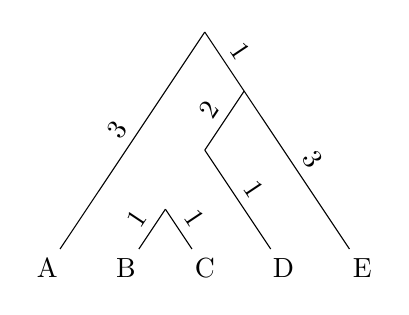
\begin{tikzpicture}
\pgftransformscale{.25}
   \node at (8,-12)  (E) {E};
   \node at (4,-12)  (D) {D};
   \node at (0,-12)  (C) {C};
    \node at (-4,-12)  (B) {B};
    \node at (-8,-12)  (A) {A};
    \draw (0,0)   -- (A) node[midway,sloped,above] {3};
    \draw (0,0)   -- (2,-3) node[midway,sloped,above] {1};
    \draw (2,-3)   -- (E) node[midway,sloped,above] {3};
    \draw (2,-3)   -- (0,-6) node[midway,sloped,above] {2};
   \draw (0,-6)   -- (D) node[midway,sloped,above] {1};
   \draw (-2,-9)   -- (C) node[midway,sloped,above] {1};
   \draw (-2,-9)   -- (B) node[midway,sloped,above] {1};
    \end{tikzpicture}
    \subcaption{$\{B,C \mid A,D,E\}$}
   \end{subfigure}
    \caption{Non-trivial splits of $T_1$.}
    \label{fig:splitst1}
\end{figure}




\begin{figure}[H]
      \begin{subfigure}[t]{0.45\textwidth}
   \centering
        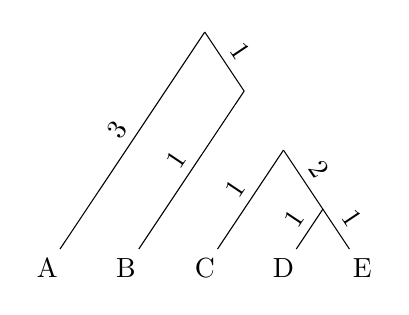
\begin{tikzpicture}
    
\pgftransformscale{.25}
   \node at (8,-12)  (E) {E};
   \node at (4,-12)  (D) {D};
   \node at (0,-12)  (C) {C};
    \node at (-4,-12)  (B) {B};
    \node at (-8,-12)  (A) {A};

    
    \draw (0,0)   -- (A) node[midway,sloped,above] {3};
  
    \draw (0,0)   -- (2,-3) node[midway,sloped,above] {1};
     \draw (4,-6)   -- (6,-9) node[midway,sloped,above] {2};
     \draw (6,-9)   -- (E) node[midway,sloped,above] {1};
 
     
   \draw (6,-9)   -- (D) node[midway,sloped,above] {1};
   
   \draw (4,-6)   -- (C) node[midway,sloped,above] {1};
   \draw (2,-3)   -- (B) node[midway,sloped,above] {1};

    \end{tikzpicture}
    \subcaption{$\{A,B \mid C,D,E\}$}
   \end{subfigure}
\hfill
  \begin{subfigure}[t]{0.45\textwidth}
   \centering
        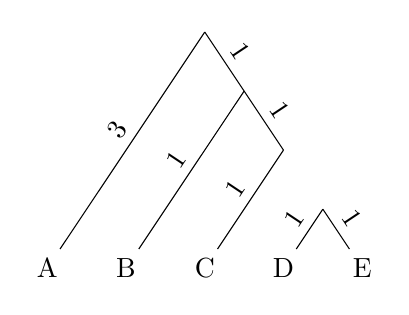
\begin{tikzpicture}
    
\pgftransformscale{.25}
   \node at (8,-12)  (E) {E};
   \node at (4,-12)  (D) {D};
   \node at (0,-12)  (C) {C};
    \node at (-4,-12)  (B) {B};
    \node at (-8,-12)  (A) {A};

    
    \draw (0,0)   -- (A) node[midway,sloped,above] {3};
  
    \draw (0,0)   -- (2,-3) node[midway,sloped,above] {1};
     \draw (2,-3)   -- (4,-6) node[midway,sloped,above] {1};
     \draw (6,-9)   -- (E) node[midway,sloped,above] {1};

   \draw (6,-9)   -- (D) node[midway,sloped,above] {1};
   
   \draw (4,-6)   -- (C) node[midway,sloped,above] {1};
   \draw (2,-3)   -- (B) node[midway,sloped,above] {1};

    \end{tikzpicture}
    \subcaption{$\{A,B,C \mid D,E\}$}
   \end{subfigure}

    \caption{Non-trivial splits of $T_2$.}
    \label{fig:splitst2}
\end{figure}

The number of splits not shared between two trees. \\
$T$ and $T_1$ share one split and each have a unique split. Therefore: 
\[
d_{symmetric} (T, T_1 ) = 2
\]
The same is true for $T$ and $T_2$. Therefore:
\[
d_{symmetric} (T, T_2 ) = 2
\]
\subsection{Quartets distance}
\begin{table}[H]
    \centering
    \begin{tabular}{c|ccccc}
        Tree & $\{A,B,C,D\}$ & $\{A,B,C,E\}$ & $\{A,B,D,E\}$ & $\{A,C,D,E\}$ & $\{B,C,D,E\}$     \\ \hline
       $T$  & $(A,D),(B,C)$ & $(A,E),(B,C)$ & $(A,B),(D,E)$ & $(A,C),(D,E)$ & $(C,B),(D,E)$ \\
       $T_1$  & $(A,D),(B,C)$ & $(A,E),(B,C)$ &\textcolor{red}{ $(A,E),(B,D)$} & \textcolor{red}{$(A,E),(C,D)$} & $(C,B),(D,E)$ \\
       $T_2$  & \textcolor{red}{$(A,B),(C,D)$} & \textcolor{red}{$(A,B),(C,E)$} & $(A,B),(D,E)$ & $(A,C),(D,E)$ & $(C,B),(D,E)$ 
    \end{tabular}
    \caption{Realization of quartet subtrees.}
    \label{tab:my_label}
\end{table}
$T$ and $T_1$ share three quartets and have two uniquely realized ones. Therefore: 
\[
d_{Quartet} (T, T_1 ) = \frac{2}{5}
\]
The same is true for $T$ and $T_2$. Therefore:
\[
d_{Quartet} (T, T_2 ) = \frac{2}{5}
\]
\section{Robinson-Foulds distance}
\begin{table}[H]
\centering
\begin{tabular}{l|cc|c}
\textbf{Split} & \multicolumn{2}{c|}{\textbf{Branch lengths ($T \mid T_1$)}} & \textbf{Difference} \\
\hline
$\{A \mid B,C,D,E\}$ & 6 & 4 & 2 \\ 
$\{B \mid B,C,D,E\}$ & 2 & 1 & 1 \\
$\{C \mid A,B,D,E\}$ & 2 & 1 & 1 \\
$\{D \mid A,B,C,E\}$ & 2 & 1 & 1 \\
$\{E \mid A,B,C,D\}$ & 2 & 3 & 1 \\
% T
$\{A,B,C \mid D,E\}$ & 5 & 0 & 5 \\
$\{B,C \mid A,D,E\}$ & 4 & 1 & 3 \\
% T1
$\{A,E \mid B,C,D\}$ & 0 & 2 & 2 \\
\hline
\textbf{Total} & & & \textbf{16???(falsch)} \\
\end{tabular}
\end{table}
\begin{table}[H]
\centering
\begin{tabular}{l|cc|c}
\textbf{Split} & \multicolumn{2}{c|}{\textbf{Branch lengths ($T \mid T_2$)}} & \textbf{Difference} \\
\hline
$\{A \mid B,C,D,E\}$ & 6 & 4 & 2 \\ 
$\{B \mid B,C,D,E\}$ & 2 & 1 & 1 \\
$\{C \mid A,B,D,E\}$ & 2 & 1 & 1 \\
$\{D \mid A,B,C,E\}$ & 2 & 1 & 1 \\
$\{E \mid A,B,C,D\}$ & 2 & 1 & 1 \\
% T
$\{A,B,C \mid D,E\}$ & 5 & 2 & 3 \\
$\{B,C \mid A,D,E\}$ & 4 & 0 & 4 \\
% T2
$\{A,B \mid C,D,E\}$ & 0 & 1 & 1 \\
\hline
\textbf{Total} & & & \textbf{14???(falsch)} \\
\end{tabular}
\end{table}
